% =====================================================
%  FinFET〜CFET構造進化チュートリアル論文(日本語版 / IEEEスタイル)
% =====================================================

\documentclass[conference]{IEEEtran}

% -----------------------------------------------------
% パッケージ設定
% -----------------------------------------------------
\usepackage[utf8]{inputenc}
\usepackage[T1]{fontenc}
\usepackage{xeCJK}            % 日本語対応
\setCJKmainfont{IPAexMincho}  % 明朝体
\usepackage{graphicx}
\usepackage{amsmath,amssymb}
\usepackage{siunitx}
\usepackage{booktabs}
\usepackage{hyperref}
\usepackage{url}
\usepackage{cite}

\usepackage{tikz}
\usetikzlibrary{patterns,arrows.meta,positioning,fit}
\usepackage{tabularx}   % 表の自動幅調整

% -----------------------------------------------------
% タイトルと著者情報
% -----------------------------------------------------
\title{FinFET〜CFET構造進化チュートリアル:\\
スケーリング臨界と構造信頼性設計}

\author{%
  \IEEEauthorblockN{三溝 真一 (Shinichi Samizo)}%
  \IEEEauthorblockA{独立系半導体研究者(元セイコーエプソン) / Independent Semiconductor Researcher (ex-Seiko Epson)\\%
  Email: \href{mailto:shin3t72@gmail.com}{shin3t72@gmail.com}\quad
  GitHub: \url{https://github.com/Samizo-AITL}}%
}

% -----------------------------------------------------
% ドキュメント開始
% -----------------------------------------------------
\begin{document}
\maketitle

% -----------------------------------------------------
% 要旨(Abstract)
% -----------------------------------------------------
\begin{abstract}
\textbf{(日本語要旨)}  
本稿は、130\,nm以降におけるCMOSスケーリング技術の構造的進化を体系的に整理したチュートリアル論文である。  
プレーナーCMOSの限界を出発点として、FinFET、Gate-All-Around(GAA: Nanosheet)、そしてComplementary FET(CFET)へと至る  
構造変遷を、電界制御、熱対称性、電源分離、再現性設計の観点から俯瞰する。  
さらに、High-$k$/Metal Gate(HKMG)技術、BEOL配線スケーリング(Low-$k$絶縁膜、Dual Damascene、Backside Power Rail)および  
BSIM-CMGモデリングを統合し、微細化の最終段階における  
「\textbf{構造そのものが信頼性設計パラメータとなる時代}」の到来を示す。  
本稿は、プロセス・デバイス・回路の各階層を横断した次世代CMOS設計のための統合的指針を提供することを目的とする。  

\medskip
\textbf{(English Abstract)}  
This tutorial paper systematically reviews the structural evolution of CMOS scaling technology beyond the 130\,nm node.  
Starting from the limitations of planar CMOS, it examines the progression toward FinFET, Gate-All-Around (GAA: Nanosheet),  
and finally Complementary FET (CFET) architectures, from the perspectives of electrostatic control, thermal symmetry,  
power-rail separation, and reproducibility in device design.  
Furthermore, it integrates High-$k$/Metal Gate (HKMG) technology, BEOL scaling  
(Low-$k$ dielectrics, Dual Damascene, and Backside Power Rail), and BSIM-CMG compact modeling,  
demonstrating the paradigm in which \textbf{device structure itself becomes the design parameter of reliability}.  
The paper aims to provide unified design insights across process, device, and circuit domains  
for reliability-aware, next-generation CMOS integration.
\end{abstract}

% -----------------------------------------------------
% キーワード(Keywords)
% -----------------------------------------------------
\begin{IEEEkeywords}
FinFET, GAA, CFET, HKMG, BEOL, Backside Power Rail, BSIM-CMG, Thermal Symmetry, Structural Reliability, CMOS Scaling
\end{IEEEkeywords}

% -----------------------------------------------------
% 本文章構成
% -----------------------------------------------------
% ============================================================
% 1. はじめに
% ============================================================
\section{はじめに}

現代の複合システム設計では,構造・材料・熱・応力・電磁・信頼性といった
物理的現象の解析と,PID・状態遷移・AI制御などの制御系設計が
分離して進められることが多い。
この分離は,設計階層間の情報不整合を招き,
再解析やパラメータ再設定の繰り返しによる開発遅延や信頼性劣化を引き起こす主要因となっている。

従来の設計支援システムやEDAツールは,
個々の領域(回路,熱,応力,信号,制御など)における最適化や解析精度の向上には寄与するが,
設計全体を貫通的に接続する統合的な情報管理機構を欠いている。
そのため,ある領域での設計更新が他領域へ自動的に反映されず,
設計の一貫性と制御安定性を同時に保証することが難しい。

本研究では,この問題を解決するために,
設計・解析・制御を統一スキーマ上で接続する
新しい工学的アーキテクチャ \textbf{SystemDK with AITL Core} を提案する。
SystemDK(System Design Kernel)は,
仕様策定,制御系設計,FPGA/ASIC回路設計,構造設計,
および FEM/ノイズ解析を統合的に結合する設計基盤である。
これにより,制御モデルと物理構造が同一データ空間で連携し,
設計更新が即時に制御・解析へ伝搬する閉ループ設計環境を実現する。

さらに,AITL(Adaptive Intelligent Tri-Layer)は,
PID・FSM・LLMの三層制御構造から構成される。
PID層は物理系の実時間安定化を担い,
FSM層は動作モードと状態遷移を管理し,
LLM層は設計データ間の形式的整合性を監督する。
AITLはSystemDKの中核制御系として動作し,
設計フロー全体を安定化させる自律的な制御基盤を形成する。

本論文では,SystemDK with AITL Coreの
統合設計フロー,制御理論,および信頼性統合手法を体系的に示す。
提案する設計体系は,仕様策定から実装検証までの全工程を閉ループで連携させ,
物理的安定性と情報的整合性を同時に保証する
自律的設計アーキテクチャの基礎をなすものである。

\section{プレーナーMOS構造の限界}
プレーナーMOSFETにおいては、チャネル長の短縮に伴い、ドレイン電界がチャネル領域へ深く侵入する短チャネル効果(SCE: Short Channel Effect)が顕著化する。  
その結果、しきい値電圧($V_{\mathrm{th}}$)の低下、ドレイン誘起バリア低下(DIBL: Drain-Induced Barrier Lowering)、およびサブスレッショルド領域における漏れ電流特性の劣化が発生する。  
これらの現象は、チャネルポテンシャルの空間的制御がドレイン電位に依存することに起因しており、従来の二次元電界近似では十分に説明できない領域に突入したことを示している。

130\,nm世代以降では、ゲート酸化膜厚が数\si{\nano\meter}領域に達し、酸化膜のトンネル電流が支配的となった。  
酸化膜を薄膜化してしきい値電圧を維持しようとすると、ゲートリーク電流が指数関数的に増大し、絶縁破壊耐性が急激に低下する。  
これにより、単なるスケーリング則(Dennard則)に基づく寸法縮小はもはや成立せず、電界分布そのものを三次元的に制御する新構造の必要性が生じた。

この臨界点において登場したのが、立体的なチャネル構造を持つFinFETである。  
FinFETは、シリコン基板上に垂直フィンを形成し、ゲートを三方向から包み込むことでチャネル電界制御を強化し、SCEおよびDIBLを抑制した。  
この構造的転換は、MOSFET動作を「面制御」から「体積制御」へと拡張するものであり、  
以後のGAA(Gate-All-Around)およびCFET(Complementary FET)へと続く三次元構造進化の出発点となった。

\section{FinFET構造とその特徴}
FinFETは、立体的に形成されたシリコンフィン(Fin)をゲートが三方向から包み込む立体チャネル構造を有する。  
この三面ゲート構造により、チャネル電位の空間分布を高精度に制御でき、プレーナーMOSFETに比べてドレイン電界の侵入を大幅に抑制する。  
結果として、短チャネル効果(SCE)の緩和、ドレイン誘起バリア低下(DIBL)の低減、サブスレッショルドスイング(SS)の改善が同時に達成される。

Fin構造の幾何学的パラメータは、電気特性を直接支配する。  
Finの高さを$H$、幅を$W$、Fin数を$n$とすると、有効チャネル幅$W_{\mathrm{eff}}$は次式で表される:
\begin{equation}
W_{\mathrm{eff}} = n(2H + W).
\end{equation}
この式は、側面チャネルが電流伝導に支配的であることを示し、Finの高さを増すことでドライブ能力($I_{\mathrm{ON}}$)を高められる一方、過剰な高さは機械的強度やエッチング制御の面で限界をもたらす。

FinFETの主な利点は、(1)ゲート制御性の向上、(2)オフリーク電流の低減、(3)動作電圧の低下による低消費電力化である。  
一方で、製造上の課題として、Fin寸法の微小ばらつき(Line Edge Roughness, LER)やゲート包囲部の非対称性がしきい値電圧$V_{\mathrm{th}}$の揺らぎを引き起こし、デバイス間の性能均一性を制限する。  
さらに、高アスペクト比Fin構造では、ゲート酸化膜堆積やメタルゲート充填における段差被覆性(Step Coverage)が信頼性を支配する要因となる。

このようにFinFETは、平面構造の限界を克服するだけでなく、デバイス設計における「電界制御性とプロセス均一性の最適折衷」を追求する新たな設計パラダイムを提示した。  
次章では、このFin構造をさらに発展させた全包囲ゲート構造GAA(Gate-All-Around)について述べる。

% (FinFET節の本文のすぐ後ろ)
\begin{table}[t]
  \centering
  \caption{FinFET代表パラメータ例(概念値)}
  \label{tab:finfet_params}
  \setlength{\tabcolsep}{4pt}
  \renewcommand{\arraystretch}{1.1}
  \small
  \begin{tabularx}{\linewidth}{l c c X}
    \toprule
    パラメータ & 記号 & 代表値 & 備考 \\
    \midrule
    Fin高さ & $H$ & 40--60\,nm & 電流駆動へ強く寄与 \\
    Fin幅   & $W$ & 5--10\,nm & SCE/SSに影響(過小でR上昇) \\
    Fin数   & $n$ & 2--4 & セル幅・ばらつきとトレード \\
    有効チャネル幅 & $W_\mathrm{eff}$ & $n(2H+W)$ & 実効伝導面積(側面優位) \\
    しきい値電圧 & $V_\mathrm{th}$ & 0.35--0.45\,V & LER・ゲートワーク関与 \\
    オン電流 & $I_\mathrm{ON}$ & $\sim$1\,mA/$\mu$m & 高$H$/小$W$で増加 \\
    オフ電流 & $I_\mathrm{OFF}$ & $<100$\,pA/$\mu$m & 三面ゲートで抑制 \\
    サブスレッショルド & $SS$ & 65--75\,mV/dec & SCE抑制指標 \\
    \bottomrule
  \end{tabularx}
\end{table}

\begin{figure}[t]
  \centering

  % ---------- TikZ Styles ----------
  \tikzset{
    gate/.style   ={pattern=north east lines, pattern color=black, draw=black, line width=0.3pt},
    oxide/.style  ={fill=black!8, draw=black, line width=0.3pt},
    si/.style     ={fill=white, draw=black, line width=0.4pt},
    sd/.style     ={fill=black!25, draw=black, line width=0.3pt},
    substrate/.style={fill=black!15, draw=black, line width=0.3pt},
    label/.style  ={font=\footnotesize},
    dim/.style    ={-{Latex[length=2mm]}, line width=0.3pt}
  }

  % ---------- Drawing ----------
  \begin{tikzpicture}[scale=1.05]

    % Substrate
    \draw[substrate] (-0.5,0) rectangle (4.5,-0.5);
    \node[label] at (2.0,-0.8) {Substrate};

    % STI / isolation background
    \draw[oxide] (0,0) rectangle (4,1.5);

    % Fin (Si)
    \draw[si] (1.75,0) rectangle (2.25,1.2);

    % Gate oxide (thin)
    \draw[oxide] (1.65,0) rectangle (2.35,1.22);

    % Gate electrode (3 sides)
    \draw[gate] (1.35,0.2) rectangle (2.65,1.15);

    % Source / Drain
    \draw[sd] (0.25,0.2) rectangle (1.35,1.15);
    \draw[sd] (2.65,0.2) rectangle (3.75,1.15);

    % Labels (non-overlapping)
    \node[label] at (0.8,1.35) {Source (S)};
    \node[label] at (3.2,1.35) {Drain (D)};
    \node[label,align=center] at (2.0,1.4) {Gate};
    \node[label] at (2.0,0.6) {Fin (Si)};

    % Dimension arrows
    \draw[dim] (1.75,0.0) -- ++(0,1.2) node[midway,left=2pt,label] {$H$};
    \draw[dim] (1.75,1.25) -- ++(0.5,0) node[midway,above=2pt,label] {$W$};

  \end{tikzpicture}

  % ---------- Caption ----------
  \caption{FinFETの断面模式図(高精細版)。ゲート電極は三面を包囲し、Finの幾何パラメータ $H,\,W$ は有効チャネル幅 $W_{\mathrm{eff}} = n(2H + W)$ に寄与する。}
  \label{fig:finfet_detail}
\end{figure}


\section{GAA(Gate-All-Around)構造}
GAA(Gate-All-Around)構造は、チャネルを全周囲からゲート電極で包み込むことにより、静電制御性を極限まで高めたデバイス構造である。  
従来のFinFETではゲートが三方向からチャネルを制御していたのに対し、GAAでは上下方向にもゲート電界が作用するため、  
チャネルポテンシャルの均一性が飛躍的に向上し、ドレイン電界の侵入がほぼ完全に抑制される。  
これにより、短チャネル効果(SCE)およびドレイン誘起バリア低下(DIBL)がさらに低減され、  
しきい値電圧$V_{\mathrm{th}}$の安定性とサブスレッショルドスイング(SS)の改善が同時に達成される。

ナノシート型GAA構造では、複数のチャネル層(Nanosheet)を垂直方向に積層し、それぞれを独立にゲートで包囲する。  
この積層構造により、平面面積を増加させずに実効チャネル幅を拡大できる。  
有効チャネル幅$W_{\mathrm{eff}}$はFinFET構造に対して次式で表される:
\begin{equation}
  W_{\mathrm{eff}} = 2n(H + W),
\end{equation}
ここで$n$はチャネル層数、$H$はシート厚、$W$はチャネル幅である。  
この式が示すように、GAAではFinFETと異なり上下両面に電流経路が追加されるため、  
同一フットプリントでより高い駆動能力を実現できる。

さらにGAA構造は「構造的スケーラビリティ」を備えており、チャネル幅$W$を減少させながら層数$n$を増やすことで、  
電気的特性を維持したまま幾何学的スケーリングを継続できる。  
この特性により、IMECやSamsungをはじめとする研究機関・メーカーでは、5\,nm世代以降でのGAA採用を加速させ、  
1.4\,nmクラスのノードにおいてもチャネル制御性と電流駆動性能の両立が実現されつつある。

一方で、ナノシートの積層・分離工程には極めて高い製造精度が要求される。  
層間酸化膜の厚さ均一性、ゲート堆積時の段差被覆性、およびチャネル層のエッチング選択性は、  
いずれもデバイス信頼性に直結する重要因子である。  
これらの課題に対処するため、Selective Epitaxial Growth(SEG)によるチャネル形成や、  
Atomic Layer Deposition(ALD)による高均一絶縁膜堆積技術が適用されている。

GAAは、FinFETの静電制御性を極限まで拡張した「完全電界包囲デバイス」として、  
次世代スケーリングの中核技術を形成している。  
次章では、n型およびp型デバイスを垂直方向に積層したCFET(Complementary FET)構造について、  
その統合アーキテクチャと設計上の課題を論じる。

\begin{table}[t]
  \centering
  \caption{GAA(Gate-All-Around)ナノシート構造の代表パラメータ\\
  Representative Parameters of GAA Nanosheet Structure}
  \label{tab:gaa_params}
  \setlength{\tabcolsep}{3pt}       % 列間やや広く
  \renewcommand{\arraystretch}{1.15}% 行間ゆとり
  \small                            % 通常より少し小さめ(視認性確保)
  \resizebox{\columnwidth}{!}{      % 幅は自動で調整
  \begin{tabular}{lccc}
    \toprule
    パラメータ & 記号 & 代表値 & 備考 \\[-3pt]
    Parameter & Symbol & Typical Value & Remarks \\
    \midrule
    ナノシート層数 & $n$ & 3--5 &
      \begin{tabular}[c]{@{}l@{}}積層により有効チャネル幅$W_\mathrm{eff}$が増大\\
      Stacking increases $W_\mathrm{eff}$\end{tabular} \\
    シート厚 & $T_s$ & 5--8\,nm &
      \begin{tabular}[c]{@{}l@{}}チャネル厚制御が性能を支配\\
      Channel thickness dominates performance\end{tabular} \\
    シート間距離 & $S$ & 10--12\,nm &
      \begin{tabular}[c]{@{}l@{}}熱干渉と寄生容量に影響\\
      Affects thermal and parasitic coupling\end{tabular} \\
    有効チャネル幅 & $W_\mathrm{eff}$ & $2n(H+W)$ &
      \begin{tabular}[c]{@{}l@{}}全包囲ゲート寄与を反映\\
      Reflects all-around gate contribution\end{tabular} \\
    しきい値電圧 & $V_\mathrm{th}$ & 0.35--0.40\,V &
      \begin{tabular}[c]{@{}l@{}}対称構造で制御容易\\
      Symmetric structure allows easy control\end{tabular} \\
    サブスレッショルド特性 & $SS$ & 60--65\,mV/dec &
      \begin{tabular}[c]{@{}l@{}}理想スイングに近似\\
      Near-ideal subthreshold swing\end{tabular} \\
    電流駆動比 & $I_\mathrm{ON}/I_\mathrm{OFF}$ & 2--3× &
      \begin{tabular}[c]{@{}l@{}}FinFET比で高駆動効率\\
      2–3× drive gain over FinFET\end{tabular} \\
    \bottomrule
  \end{tabular}
  } % end resizebox
\end{table}

% =====================================================
% Fig. 6 : GAA(Gate-All-Around)ナノシート構造 断面図
% =====================================================
\begin{figure}[t]
  \centering
  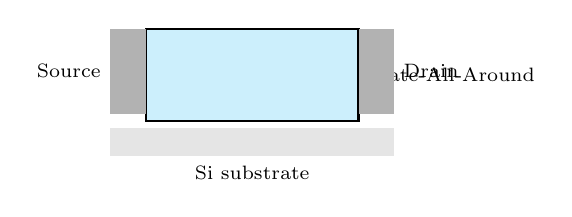
\begin{tikzpicture}[scale=0.9, every node/.style={font=\scriptsize}]
    % substrate
    \fill[gray!20] (0,0) rectangle (4,0.4);
    \node[below] at (2,0) {Si substrate};

    % nanosheets (3層)
    \foreach \y in {0.6,1.0,1.4} {
      \fill[orange!30] (0.8,\y) rectangle (3.2,\y+0.2);
      \draw[black!50] (0.8,\y) rectangle (3.2,\y+0.2);
    }

    % gate stack
    \draw[thick,fill=cyan!20] (0.5,0.5) rectangle (3.5,1.8);
    \node[right] at (3.55,1.15) {Gate-All-Around};

    % source/drain
    \fill[gray!60] (0,0.6) rectangle (0.5,1.8);
    \fill[gray!60] (3.5,0.6) rectangle (4.0,1.8);
    \node[left] at (0,1.2) {Source};
    \node[right] at (4,1.2) {Drain};
  \end{tikzpicture}

  \caption{GAAナノシート構造の模式断面図(S/D領域とゲート包囲面を示す)\\
  \footnotesize Schematic cross-section of GAA nanosheet structure showing gate wrapping around multiple stacked channels.}
  \label{fig:gaa_cross}
\end{figure}


\section{CFET(Complementary FET)構造}
CFET(Complementary Field-Effect Transistor)は、n型およびp型のトランジスタを垂直方向に積層した三次元デバイス構造であり、  
従来の平面配置(lateral arrangement)から垂直配置(vertical stacking)への構造転換を特徴とする。  
このアプローチにより、トランジスタ・セルが占有する平面面積を大幅に削減し、  
同一チップ面積あたりの集積度をFinFETやGAA構造を超えて向上させることが可能となる。

CFETでは、nFETとpFETが上下に積層され、それぞれ独立したゲートおよびソース/ドレイン構造を持つ。  
この垂直積層構造により、同一セル内で上下デバイスが相補的に動作するため、  
標準セル高さを縮小しながら論理駆動能力を維持できる。  
さらに、Backside Power Rail(BPR)技術との統合が容易であり、  
信号線と電源線の物理的分離によって配線抵抗および寄生結合を低減し、電源ノイズ耐性を向上させる。

GAA技術をベースとするCFETでは、上下のトランジスタを独立に電気的制御する必要があるため、  
チャネル層間のアイソレーション精度および熱干渉の抑制が設計上の要点となる。  
n型とp型デバイスが異なる移動度・発熱特性を有する場合、  
垂直方向の熱対称性(thermal symmetry)が支配因子となり、  
電流駆動能力および信頼性(NBTI/HCI耐性)に直接影響を及ぼす。

製造上の課題としては、垂直積層におけるソース/ドレインの選択的エピタキシャル成長、  
層間絶縁膜(Inter-Layer Dielectric; ILD)の平坦化精度、  
およびn/pトランジスタ間の電気的アイソレーション確保が挙げられる。  
特に、上部デバイス形成後に下部デバイス特性が劣化しないよう、  
プロセス全体の低温化($<400\,^{\circ}\mathrm{C}$)が不可欠である。  
このため、Selective EpitaxyやLow-Temperature ALDによるメタルゲート堆積など、  
熱負荷を最小限に抑えるプロセス技術が開発されている。

CFETは、GAAを超えて「論理対称性と物理空間効率の両立」を実現する究極の三次元CMOSアーキテクチャである。  
現在、IMEC、Intel、Samsungなどの主要研究機関・メーカーが試作段階に到達しており、  
1\,nmクラス以降のロジックデバイスにおける有力な主流候補と位置付けられている。  
次章では、こうした三次元構造を支える配線および電源インテグレーション技術(BEOLおよびBPR)について論じる。

\begin{table}[t]
  \centering
  \caption{CFET(Complementary FET)構造設計パラメータ}
  \label{tab:cfet_stack}
  \begin{tabular}{lccc}
    \toprule
    項目 & 記号 & 代表値 & 備考 \\
    \midrule
    n/p積層距離 & $d_{np}$ & 20–30\,nm & 熱干渉最小化に設計 \\
    上部チャネル厚 & $T_p$ & 5–7\,nm & pFET層 \\
    下部チャネル厚 & $T_n$ & 5–7\,nm & nFET層 \\
    絶縁層厚 & $T_\mathrm{ILD}$ & 10\,nm & 熱・電気分離層 \\
    BPR金属厚 & $T_\mathrm{BPR}$ & 100–150\,nm & 電源層再配置 \\
    電源分離効率 & $\eta_\mathrm{BPR}$ & $>$90\% & IRドロップ低減効果 \\
    面積削減率 & $A_\mathrm{red}$ & 35–40\% & FinFET比 \\
    \bottomrule
  \end{tabular}
\end{table}

% =====================================================
% Fig. 7 : CFET(Complementary FET)垂直積層構造 断面図
% =====================================================
\begin{figure}[t]
  \centering
  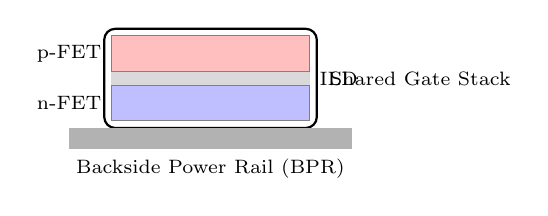
\begin{tikzpicture}[scale=0.9, every node/.style={font=\scriptsize}]
    % bottom n-FET
    \fill[blue!25] (0.6,0.4) rectangle (3.4,0.9);
    \draw[black!50] (0.6,0.4) rectangle (3.4,0.9);
    \node[left] at (0.6,0.65) {n-FET};

    % isolation (ILD)
    \fill[gray!30] (0.6,0.9) rectangle (3.4,1.1);
    \node[right] at (3.4,1.0) {ILD};

    % top p-FET
    \fill[red!25] (0.6,1.1) rectangle (3.4,1.6);
    \draw[black!50] (0.6,1.1) rectangle (3.4,1.6);
    \node[left] at (0.6,1.35) {p-FET};

    % gate stack
    \draw[thick,rounded corners] (0.5,0.3) rectangle (3.5,1.7);
    \node[right] at (3.55,1.0) {Shared Gate Stack};

    % backside power rail (BPR)
    \fill[gray!60] (0,0) rectangle (4,0.3);
    \node[below] at (2,0) {Backside Power Rail (BPR)};
  \end{tikzpicture}

  \caption{CFET構造の垂直積層模式図(n/pスタックおよびBPRを示す)\\
  \footnotesize Schematic vertical stack of CFET showing n/p layers and backside power rail.}
  \label{fig:cfet_cross}
\end{figure}


\section{BEOL(配線技術)の進化}
デバイススケーリングと並行して、BEOL技術も大きく進化した。  
Low-k誘電体と銅配線の導入によりRC遅延を低減し、Dual Damasceneプロセスにより高密度配線を実現した。  
7\,nm以降では、BPR(Backside Power Rail)により電源層をシリコン裏面側に再配置し、セル内部配線の自由度を拡大している。

\section{スケーリングパラメータの推移}
トランジスタの微細化は長年にわたり、いわゆる「Dennardスケーリング則」に基づいて進展してきた。  
この比例則は、チャネル長、酸化膜厚、電源電圧を一定比率で同時に縮小することで、  
トランジスタ性能を維持しながら消費電力を低減できるという理論的基盤を提供してきた。  
しかし、90\,nm世代以降、リーク電流および電界強度の増大によりこの単純なスケーリング則は破綻し、  
電気的・構造的な最適化を同時に考慮する新しいパラダイムが必要となった。

この技術的変遷を俯瞰するために、表\ref{tab:process_evolution}に主要プロセスノードにおける  
**構造的および材料的進化(Process Revolution)** を示す。  
同表に見られるように、電源電圧$V_{DD}$は130\,nm世代の1.2\,Vから2\,nm世代ではおよそ0.6\,Vへと低下し、  
一方でゲート酸化膜厚$T_\text{ox}$および実効酸化膜厚(EOT)は1\,nm前後にまで到達している。  
この臨界領域では、トンネルリークが支配的となるため、High-$k$/Metal Gate(HKMG)技術が導入された。  
HKMGは実効EOTを維持しつつリーク電流$I_\text{G}$を数桁低減し、  
FinFETおよびGAA構造への橋渡し技術として機能している。

さらに、FinFETおよびGAA構造の採用により、ゲート電界による静電制御性が飛躍的に向上した。  
電源電圧の低下に伴う駆動電流$I_\text{ON}$の減少は、チャネル形状の立体化と高移動度材料の導入によって補償されている。  
このように、「スケーリングの限界」は単なる寸法縮小の限界ではなく、  
**構造変革(Structural Revolution)** としてのスケーリング再定義を意味している。

今後のCFET世代以降では、以下のような多次元設計最適化が求められる:
\begin{itemize}
    \item 高移動度チャネル材料(SiGe, Ge, III–V族)による$I_\text{ON}/I_\text{OFF}$改善  
    \item Backside Power Rail(BPR)および低抵抗BEOLによる電圧降下抑制  
    \item 多層絶縁膜スタックによる電界集中の緩和  
\end{itemize}
これらにより、スケーリングは幾何学的寸法値ではなく、  
**「電気的・熱的・構造的最適化空間」** の設計パラメータとして再定義されつつある。

\begin{table*}[t]
  \centering
  \caption{CMOSスケーリングにおけるプロセス構造の進化(Process Evolution of CMOS Scaling)}
  \label{tab:process_evolution}
  \scriptsize
  \setlength{\tabcolsep}{4pt}
  \renewcommand{\arraystretch}{1.1}
  \begin{tabular}{ccccccc}
    \toprule
    ノード & 構造 & 電源電圧[V] & $T_\mathrm{ox}$[nm] & Min L[nm] & 主な特徴 & 技術課題 \\
    Node & Structure & $V_\mathrm{DD}$[V] & $T_\mathrm{ox}$[nm] & Min L[nm] & Key Features & Challenges \\
    \midrule
    90\,nm & プレーナMOS & 1.2 & $\sim$2.0 & $\sim$65 & NiSi導入、Strained-Si、LDD最適化 & リーク電流、寄生容量、リソグラフィ限界 \\
           & Planar MOS &     &              &           & NiSi, strained-Si, optimized LDD & Leakage, parasitics, lithography \\[2pt]
    45\,nm & プレーナMOS & 1.0 & $\sim$1.3 & $\sim$35 & HKMG導入準備、ULK試験導入 & ゲート制御限界、ばらつき拡大 \\
           & Planar MOS &     &             &          & HKMG prep, ULK intro & Gate control limit, variability \\[2pt]
    22\,nm & FinFET初代 & 0.85 & $\sim$0.9 & $\sim$20 & Tri-Gate構造採用、3Dチャネル化 & Finばらつき、設計難度増加 \\
           & 1st Gen FinFET & & & & Tri-Gate, 3D channel & Fin variation, design complexity \\[2pt]
    5\,nm & GAA導入 & 0.6 & $\sim$0.6 & $\sim$8 & Nanosheet構造試験導入 & Routing困難、シート幅制御 \\
           & GAA Pilot & & & & Nanosheet trials & Sheet width control, poor routability \\[2pt]
    2\,nm & CFET試作 & $\lesssim$0.5 & $\sim$0.4 & $\sim$4 & NMOS/PMOS縦積層化 & 熱干渉、配線分離難 \\
           & CFET (R\&D) & & & & Complementary FET stacking & Thermal interference, power routing split \\
    \bottomrule
  \end{tabular}
\end{table*}


\section{BSIM-CMGモデリング}
BSIM-CMG(Berkeley Short-channel IGFET Model – Common Multi-Gate)は、  
FinFETおよびGAA(Gate-All-Around)などの非平面構造デバイスを統一的に表現するために開発された  
物理ベースSPICEコンパクトモデルである。  
従来のBSIM4モデルがプレーナーMOSFETの二次元電界分布を前提としていたのに対し、  
BSIM-CMGは三次元チャネル電位分布および多ゲート構造における電位結合(electrostatic coupling)を厳密に扱うことが可能である。

本モデルでは、チャネル電位$\psi(x,y,z)$を多変数ポアソン方程式に基づき近似的に解き、  
有効電荷密度$Q_\mathrm{inv}$およびドレイン電流$I_\mathrm{D}$をゲート電圧$V_\mathrm{G}$およびドレイン電圧$V_\mathrm{D}$の関数として定式化する:
\begin{equation}
I_\mathrm{D} =
\mu_\mathrm{eff} \, C_\mathrm{inv} \,
\frac{W_\mathrm{eff}}{L_\mathrm{g}}
(V_\mathrm{G} - V_\mathrm{th}) V_\mathrm{D}
\, f_\mathrm{sat}(E_\mathrm{ch}, T),
\end{equation}
ここで、$\mu_\mathrm{eff}$は実効キャリア移動度、$C_\mathrm{inv}$は反転層容量、  
$f_\mathrm{sat}(E_\mathrm{ch},T)$はチャネル電界および温度依存性を表す飽和関数である。  
FinFET構造では$W_\mathrm{eff}=n(2H+W)$、GAA構造では$W_\mathrm{eff}=2n(H+W)$と定義され、  
形態パラメータが直接的に電流駆動力を支配する。

BSIM-CMGはこれらの幾何学パラメータを抽象化してモデル化するため、  
FinFET、Nanosheet、Nanowireといった異なる構造間でのパラメータ再利用が可能である。  
主な制御パラメータは以下の通りである:
\begin{itemize}
    \item 実効酸化膜厚(EOT: Equivalent Oxide Thickness)  
    \item チャネル高さ$H_\mathrm{fin}$および幅$W_\mathrm{fin}$  
    \item ソース/ドレイン接合抵抗  
    \item サブスレッショルド係数$n$およびキャリア散乱係数  
    \item 温度依存項および熱ノイズ係数  
\end{itemize}
これにより、物理パラメータと回路設計変数を単一フレームで統合し、デバイス–回路協調設計(co-design)が実現される。

さらに、BSIM-CMGはチャネル内部電位を代表値で近似する「中心軸法(Core Potential Method)」を採用しており、  
非平面構造においても数値安定性と高速収束性を両立している。  
これにより、GAAやCFETのような多層チャネル構造においてもSPICEレベルの解析が安定して実行可能である。

CFETに対しては、上下トランジスタ間の電熱結合(self-heating coupling)および  
相互寄生容量を考慮した拡張モデルが提案されている。  
このモデルでは各トランジスタを独立したBSIM-CMGサブブロックとして構築し、  
電流・温度・電位の相互干渉を双方向結合させることで、  
垂直積層構造に特有の熱非対称性を高精度に再現できる。

BSIM-CMGの導入により、デバイス物理と回路設計の整合が飛躍的に向上した。  
寸法スケーリング、材料特性、熱劣化、信頼性パラメータを統一的に評価できる本モデルは、  
ポストFinFET世代における設計基盤として、構造最適化から回路レベル信頼性解析に至るまで  
広範に応用されている。  

% figs/fig_bsim_cmg_model.tex
% BSIM-CMG モデル構成図(モノクロ/外側のfigure環境は書かない)
\begin{tikzpicture}[font=\scriptsize, node distance=6mm]
  % styles
  \tikzset{
    blk/.style={draw=black, fill=black!5, rounded corners, minimum width=30mm, minimum height=7mm, align=center},
    io/.style ={draw=black, fill=black!15, rounded corners, minimum width=22mm, minimum height=7mm, align=center},
    grp/.style={draw=black, dashed, inner sep=3mm, rounded corners},
    arrow/.style={-Latex, line width=0.3pt}
  }

  % Inputs
  \node[io] (geom) {Geometry \\ (Fin/GAA params)};
  \node[io, right=of geom] (mat) {Materials \\ (EOT, $\mu$, HKMG)};
  \node[io, right=of mat] (bias) {Bias/Temp \\ ($V_G, V_D, T$)};

  % Solvers / kernels
  \node[blk, below=12mm of mat] (elec) {Electrostatics \\ (Core potential / Poisson approx.)};
  \node[blk, below=of elec] (mob) {Mobility \& Scattering \\ (phonon, surface, impurity)};
  \node[blk, below left=6mm and 7mm of mob] (sdr) {Series $R$ (S/D, contact)};
  \node[blk, below right=6mm and 7mm of mob] (sh) {Self-Heating \\ (thermal coupling)};

  % Outputs
  \node[blk, below=18mm of mob, minimum width=36mm] (charge) {Charge/Capacitance \\ ($Q$, $C_{gg}, C_{gd}, \dots$)};
  \node[blk, below=8mm of charge, minimum width=36mm] (ids) {$I_D$ Model \\ (sat. func. $f_\mathrm{sat}(E_\mathrm{ch},T)$)};

  % Group box
  \node[grp, fit=(elec) (mob) (sdr) (sh) (charge) (ids), label={[font=\footnotesize]above:BSIM-CMG Core}] (core) {};

  % Arrows: inputs -> core
  \draw[arrow] (geom.south) -- (elec.north -| geom.south);
  \draw[arrow] (mat.south)  -- (elec.north);
  \draw[arrow] (bias.south) -- (elec.north -| bias.south);

  % Flow inside core
  \draw[arrow] (elec) -- (mob);
  \draw[arrow] (mob.west) |- (sdr.north);
  \draw[arrow] (mob.east) |- (sh.north);
  \draw[arrow] (mob) -- (charge);
  \draw[arrow] (charge) -- (ids);

  % Feedbacks (dashed)
  \draw[arrow, dashed] (ids.west) |- ($(elec.south west)!0.6!(elec.north west)$);
  \draw[arrow, dashed] (sh.east)  |- ($(mob.east)+(8pt,0)$) -| (mob.east);

  % Notes
  \node[font=\scriptsize, align=left, anchor=west] at ($(core.south west)+(0, -5mm)$)
    {出力: $I_D(V_G,V_D,T)$, $Q$, 各種$C$(SPICE互換)};
\end{tikzpicture}


\section{信頼性と構造設計}
微細化の進行に伴い、デバイス信頼性は動作限界を規定する主要因となっている。  
特に、BTI(Bias Temperature Instability)、HCI(Hot Carrier Injection)、および自己発熱(Self-Heating)といった
時間依存劣化(Time-Dependent Degradation)が支配的となる。

\subsection{電界劣化と界面反応}
BTIは、ゲート酸化膜界面における電荷捕獲・放出反応に起因し、  
ゲート電圧ストレス下でしきい値電圧$V_\text{th}$が時間とともにシフトする現象である。  
特に負バイアス温度不安定性(NBTI)は$p$MOSに顕著であり、  
酸化膜中の水素脱離反応や界面欠陥生成が支配的メカニズムとされる。  
一方、HCIは高電界ドレイン領域でのキャリア加速と衝突イオン化により発生し、  
酸化膜損傷とチャネルホットキャリア蓄積を引き起こす。  
これらの現象はいずれも、電界集中と局所温度上昇の積分効果に比例して進行する。

\subsection{熱対称性と構造的緩和}
FinFETおよびGAAデバイスでは、三次元構造により放熱経路が複雑化する。  
Fin形状の側壁酸化膜は熱伝導率が低く、チャネル内で局所的な温度勾配が形成されるため、  
Self-Heating効果が移動度劣化およびBTI加速を引き起こす。  
このため、構造設計段階における「熱シンメトリ(Thermal Symmetry)」の確保が不可欠である。  
チャネル上下での温度勾配を最小化し、ゲート金属やSTI(Shallow Trench Isolation)の熱伝導経路を最適化することにより、  
局所過熱領域を抑制できる。

GAAおよびCFET構造では、チャネル層の積層により上下FET間の熱干渉が生じる。  
これに対して、下層トランジスタに高熱伝導材料(例:Geチャネル/Wゲート)を用いる、  
または熱拡散パスを金属層側に逃がす「熱ブリッジ構造(Thermal Bridge)」を設計的に導入するなど、  
構造的放熱設計が信頼性確保の中心的要素となる。

\subsection{構造信頼性設計のパラダイム}
FinFETからCFETへの進化は、単なる寸法縮小ではなく、  
「構造を通じて信頼性を設計する」という新たな設計思想への転換を意味する。  
従来は事後的に評価されていた劣化現象を、  
設計初期段階での構造パラメータ最適化により抑制するアプローチである。  
たとえば、Finピッチやゲート包囲角度、チャネル積層間距離を熱・電界分布解析と統合的に最適化することで、  
長期信頼性(Lifetime Reliability)をデザインルールの一部として保証することが可能となる。

今後は、CFETを含む垂直統合構造に対して、  
熱・電界・機械応力を同時に考慮した「マルチフィジックス信頼性設計」が必須となる。  
このように、スケーリングの最終段階では、  
**構造そのものが信頼性の設計パラメータとなる**という新たな設計パラダイムが形成されつつある。

\section{リソグラフィとマスク技術}
デバイス微細化の限界を押し広げるうえで、リソグラフィ技術の進歩は決定的な役割を果たしてきた。  
ArF液浸露光(ArF Immersion Lithography)からEUV(Extreme Ultraviolet)露光への移行は、  
露光波長の大幅短縮によって解像限界を縮小し、  
多重パターニング工程(Double/Quadruple Patterning)を劇的に削減した。  
これにより、配線ピッチの微細化に伴うプロセス変動(Overlay Error、CD Variation)が大幅に低減し、  
スループットおよび歩留まりの両立が可能となった。

\subsection{EUV露光と多重パターニング削減}
従来のArF液浸露光では、NA(Numerical Aperture)の限界により、  
40\,nm以下のパターン形成に複数回の露光・エッチングを要した。  
これに対し、13.5\,nm波長のEUV光を用いることで、  
1回の露光で30\,nmクラスのライン&スペースパターンが形成可能となった。  
この結果、工程数削減による線幅変動の抑制とともに、  
レジストパターンの位置ずれや累積誤差が大幅に緩和された。  
一方で、EUV光源の出力安定性やミラー反射損失、レジスト感度とLWR(Line Width Roughness)のトレードオフが  
次世代微細化の課題として残されている。

\subsection{マスク3D効果と光学補正}
微細パターン形成の高精度化には、マスク上の三次元効果(Mask 3D Effect)を考慮した補正設計が必須である。  
EUVマスクは多層ミラー構造を持ち、斜入射により反射位相と透過率がパターン位置によって変化する。  
このため、マスク転写像の歪みを補償するために、  
光学近接補正(OPC: Optical Proximity Correction)およびソースマスク最適化(SMO: Source Mask Optimization)が導入されている。  
これらの手法は、マスクパターン形状を露光シミュレーションと連動させ、  
最終的なシリコン上パターン精度をナノメートルスケールで保証する。

さらに、GAAおよびCFETのような三次元構造デバイスでは、  
パターン形状が深堀エッチングやゲート包囲構造と密接に関連するため、  
EUVマスク設計段階での形状歪み補正とアライメント精度がデバイス特性の再現性を左右する。  
特にCFETでは、上下層FETのゲートおよびソース・ドレインを個別に定義する必要があるため、  
多層マスク整合技術(Multi-Layer Alignment Technology)が歩留まり向上の鍵となる。

\subsection{次世代リソグラフィへの展望}
2\,nm世代以降では、High-NA EUV(開口数1.0以上)の適用が進み、  
より高い解像力とパターン忠実度を両立する見込みである。  
また、EUVペリクル(保護膜)の透過損失や、レジスト材料の化学増幅機構に起因するノイズ制限が  
量産性のボトルネックとなる可能性が指摘されている。  
これに対し、**EUVと電子線マスク補正(E-Beam Mask Repair)を組み合わせたハイブリッド露光戦略** や、  
**Computational Lithography(計算リソグラフィ)によるパターン最適化** の研究が進展している。

このように、リソグラフィとマスク技術は単なる描画プロセスではなく、  
**デバイス構造設計と一体化した「構造整合工学(Structural Lithography Engineering)」** へと進化している。  
EUV世代以降の微細化では、露光・エッチング・デバイス形状設計を統合した最適化が、  
CFET時代の高精度かつ高信頼な製造基盤を支える中心的要素となる。

\section{結論}
本稿では、130\,nm以降のCMOSスケーリングを、FinFET、GAA、そしてCFETに至る構造的進化の観点から体系的に整理した。  
プレーナーMOSの電界制御限界を突破したFinFET、完全包囲ゲート構造による静電的最適化を実現したGAA、  
そして垂直積層により論理対称性と配線効率を両立したCFETへと至る流れは、  
スケーリングの中心軸が「寸法の縮小」から「構造の最適化」へと移行したことを明確に示している。

この構造的転換は、電界・熱・信頼性といった多次元設計パラメータを同時に最適化する  
“Structure-Driven Scaling” の概念を確立したものである。  
特に、High-$k$/Metal Gate(HKMG)、Backside Power Rail(BPR)、およびBSIM-CMGモデルの統合は、  
プロセス・デバイス・回路設計を貫く一貫した設計基盤を提供し、  
信頼性と性能を両立する「構造的CMOSアーキテクチャ」を実現した。

今後のポスト-CFET時代においては、スケーリングの焦点は  
材料・構造・AIによる設計統合(AI-driven Co-Optimization)へと拡張される。  
熱対称性や電源分離構造の自動最適化、信頼性の予測設計、そして  
マルチフィジックスを考慮した構造シミュレーションが標準化されることで、  
デバイス開発は「試作依存型」から「構造駆動型知能設計」へと進化するだろう。

すなわち、**構造そのものが信頼性と性能を設計する時代**が到来しており、  
FinFET–GAA–CFETの進化はその第一歩である。  
本稿で提示した体系的整理は、次世代CMOSスケーリングにおける  
物理・設計・AI統合の指針としての基盤を提供するものである。


% -----------------------------------------------------
% 謝辞
% -----------------------------------------------------
\section*{謝辞}
本稿の作成にあたり、半導体デバイススケーリング・信頼性・プロセス統合に関して示唆に富む議論を行ってくださった
産業界および学術界の関係各位に深く感謝する。

% -----------------------------------------------------
% 参考文献
% -----------------------------------------------------
% --- force at least one item for IEEEtran ---
\nocite{*}
\bibliographystyle{IEEEtran}
\bibliography{refs}

% -----------------------------------------------------
% 著者略歴
% -----------------------------------------------------
\section*{著者略歴}
\textbf{三溝 真一}(Shinichi Samizo)は、信州大学大学院 工学系研究科 電気電子工学専攻にて修士号を取得した。  
その後、セイコーエプソン株式会社に勤務し、半導体ロジック/メモリ/高耐圧インテグレーション、  
およびインクジェット薄膜ピエゾアクチュエータならびにPrecisionCoreプリントヘッドの製品化に従事した。  
現在は独立系半導体研究者として、プロセス/デバイス教育、メモリアーキテクチャ、AIシステム統合などに取り組んでいる。  
連絡先: \href{mailto:shin3t72@gmail.com}{shin3t72@gmail.com}.

\end{document}
